% Drawing 83/10-3 -- folder 83, batch 10, archive page 200 (PDF page 201).
% Transcription: cube en perspective, avec arêtes renforcées ($a$, $\bar a$, $\bar a'$), sommets cerclés, diagonales, flèches de rotation et étiquettes $f$, $f'$, $f''$.
% Kind: cube with reinforced edges, diagonals and rotation arrows. Method 2 (schematic redraw from the facsimile). Status: partial.
% Notes: Bbox re-centred on the cube. Corners computed once, every edge drawn between the same points: the front top edge P1-P2 through the small dot M; the heavy left edge P1-BL (labelled a-bar', heavy blot at BL, drawn as a point); the heavy edge P2-P3 (a, heavy blot at P3, drawn as a point); the edge from P1 to the back corner Q drawn with cross ticks (a-bar above it); the top back edge from the ring beside Q to P3; the bottom edge BL-BR (BR ringed); the edge P2-BR with ticks; the right edge P3-R3 and the bottom right edge BR-R3; the vertical from M down to the bottom edge. Inside: the long thin line from Q down to the left, the short stroke below Q, the stroke from M up to the right (crossing the f), the hidden stroke from BL towards the back, an arc and a dashed stroke in the front face; on the right face the diagonal from P2 towards R3 (stopping short at both ends, as on the page), the diagonal rising from the edge BR-R3 and stopping short of P3-R3, and the horizontal stroke between them. Rotation arrows: on the left face (C-shaped) and under f on the top face. Labels at \small: a-bar, a-bar', a, f (top face), f' (right face, legible on this crop), f'' (front face). Still differs: the ring stands above and to the right of the corner Q where the ticked edge, the long line and the short stroke meet, and is drawn where it stands; the small asterisk on the edge P2-BR and the dashes on the hidden strokes are simplified; which corner is hidden is a reading. Redrawn 2026-11-09 (issue 128): to check again.
% Coordinates: 1 unit = 1 mm = 1/100 of the crop width (bbox in page fractions: [0.12, 0.2, 0.32, 0.31]).
% Redrawn by Claude (claude-opus-5-5), issue #73, 2026-11-09; not checked by a human; not compiled (no TeX in the session).
% Rights: reproduces part of the work -- behind RENDER_TRANSCRIPTS, never published by itself.
\documentclass[tikz,border=3pt]{standalone}
\usepackage{amsmath,amssymb}
\usetikzlibrary{patterns,arrows.meta}
\tikzset{pencil/.style={black!45}, struck/.style={black!35}, mark/.style={circle,draw,inner sep=1.3pt}, pt/.style={circle,fill,inner sep=0.9pt}, opt/.style={circle,draw,fill=white,inner sep=1.1pt}}
\begin{document}
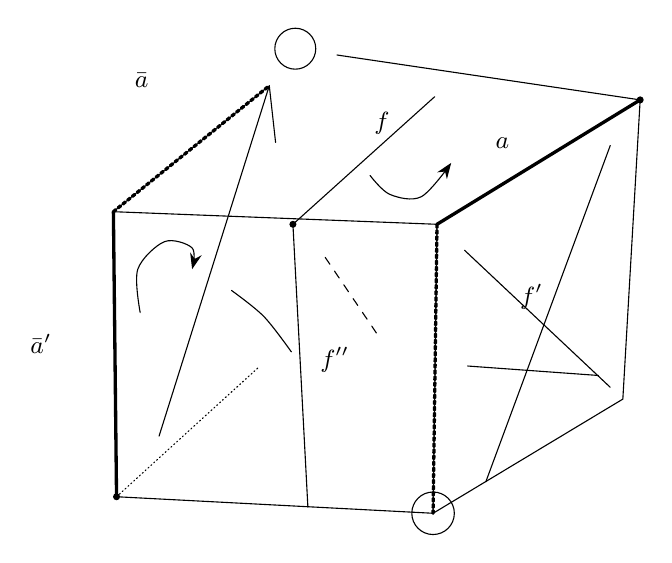
\begin{tikzpicture}[x=1mm,y=1mm,line cap=round,line join=round,font=\scriptsize]
\draw (20.4,-29.2) -- (61.5,-30.8);
\draw[very thick] (20.4,-29.2) -- (20.8,-65.4);
\draw[very thick] (61.5,-30.8) -- (87.3,-15);
\draw[densely dotted,very thick] (20.4,-29.2) -- (40.2,-13.2);
\draw (48.8,-9.3) -- (87.3,-15);
\draw (20.8,-65.4) -- (61,-67.5);
\draw[densely dotted,very thick] (61.5,-30.8) -- (61,-67.5);
\draw (87.3,-15) -- (85.1,-53);
\draw (61,-67.5) -- (85.1,-53);
\draw (43.2,-30.8) -- (45.1,-66.7);
\draw (40.2,-13.2) -- (26.2,-57.7);
\draw (40.2,-13.2) -- (41,-20.4);
\draw (43.2,-30.8) -- (61.2,-14.6);
\draw[densely dotted] (20.8,-65.4) -- (38.8,-49);
\draw plot[smooth, tension=0.55] coordinates {(35.4,-39.2) (39.5,-42.5) (43,-47)};
\draw[dashed] (47.3,-35) -- (53.8,-44.6);
\draw (65,-34.1) -- (83.5,-51.5);
\draw (67.7,-63.5) -- (83.5,-20.8);
\draw (65.4,-48.8) -- (82,-50);
\draw (43.5,-8.5) circle[radius=2.6];
\draw (61,-67.5) circle[radius=2.7];
\node[pt] at (43.2,-30.8) {};
\node[pt] at (20.8,-65.4) {};
\node[pt] at (87.3,-15) {};
\draw[-{Stealth[length=2mm]}] plot[smooth, tension=0.55] coordinates {(23.8,-42) (23.5,-36.5) (26.9,-33) (30.4,-33.8) (30.4,-36.5)};
\draw[-{Stealth[length=2mm]}] plot[smooth, tension=0.55] coordinates {(53,-24.6) (55.5,-27) (59.5,-27.3) (63.3,-23)};
\node[inner sep=1pt] at (24,-12.5) {\small $\bar a$};
\node[inner sep=1pt] at (11.2,-46) {\small $\bar a'$};
\node[inner sep=1pt] at (69.8,-20.5) {\small $a$};
\node[inner sep=1pt] at (54.5,-18) {\small $f$};
\node[inner sep=1pt] at (73.5,-40) {\small $f'$};
\node[inner sep=1pt] at (48.5,-48) {\small $f''$};
\end{tikzpicture}
\end{document}
